\documentclass[journal=esthag,manuscript=article]{achemso}

% additional packages
\usepackage[utf8]{inputenc}
\usepackage{amsmath}
\usepackage{booktabs}
\usepackage{subcaption}
\usepackage{tabularx}
\usepackage{array,multirow,graphicx}
\usepackage{comment}
\graphicspath{
  {./../figures/},
  {./../figures/air-exchange-rate/},
  {./../figures/kde-iacc-pressure/},
  {./../figures/simulation_predictions/},
  {./../figures/pair_grids/},
  {./../figures/multivariate_analysis/}
}
\usepackage{lineno}
\linenumbers
% macros

% authors
\author{Jonathan G. V. Ström}
\affiliation[Brown University]{Brown University, School of Engineering, Providence, RI, USA}
\author{Yijun Yao}
\affiliation[Zhejiang University]{Zhejiang University, Hangzhou, China}
\author{Eric M. Suuberg}
\email{eric_suuberg@brown.edu}
\affiliation[Brown University]{Brown University, School of Engineering, Providence, RI, USA}

% title
\title{Transient Variability In Vapor Intrusion And The Factors That Influence It}

% keywords
\abbreviations{VI}
\keywords{Vapor intrusion, Preferential pathways, Temporal variability, Factor analysis, Modeling}

\begin{document}

\begin{abstract}

\end{abstract}

\section{Introduction}

The significant temporal varibility in indoor air contaminant concentrations at vapor intrusion (VI) sites pose a major impedent for assertaining the relevant human exposure to vapor contaminant.
Exactly how significantly the indoor air concentration may vary, and the causes of the variability is poorly understood.
Improving our understanding of these two factors are crucial to reduce uncertainty in determining indoor air contaminant exposures, and reducing the length of these investigations.


Two well-documentated VI sites both showed significant temporal variability in indoor air contaminant concentrations.
One is a two-story house near Hill AFB in Utah (called the ASU house in this paper), and the other a duplex in Indianapolis, IN.

The discovery of preferential pathways for contaminant entry at VI sites has further

\section{Methods}

\subsection{Statistical Analysis}

This paper heavily relies on statistical analysis of high resolution datasets from two well-studied VI sites, one near Hill AFB in Utah (called the ASU house) and another in Indianapolis, IN (simply called as such.)
Analysis is performed using the SciPy, NumPy, Pandas, and Seaborn Python packages.
Probability distributions of various parameters are constructed using the kernel density estimation (KDE) method\cite{altman_introduction_1992}, which is implemented in the SciPy package.

At the Indianapolis site, we only consider the 422 side of the duplex, which was heated.
Indoor air concentration in this case, specifically refer to the indoor air contaminant concentration in the 422 basement.
Soilgas concentration refers only to samples taken from SGP2.
The indoor/outdoor pressure difference is the 422 basement and exterior pressure difference.  

The indoor/outdoor pressure difference were recorded every two minutes.
Indoor air samples were taken every four hours.

\subsection{Vapor Intrusion Model}



\section{Results & Discussion}

\subsection{Statistical Analysis of Field Data}



\begin{figure}[!h]
	\centering
	\begin{minipage}[c]{0.49\textwidth}
		\centering
    \caption{ }
    \label{fig:asu_phase}
    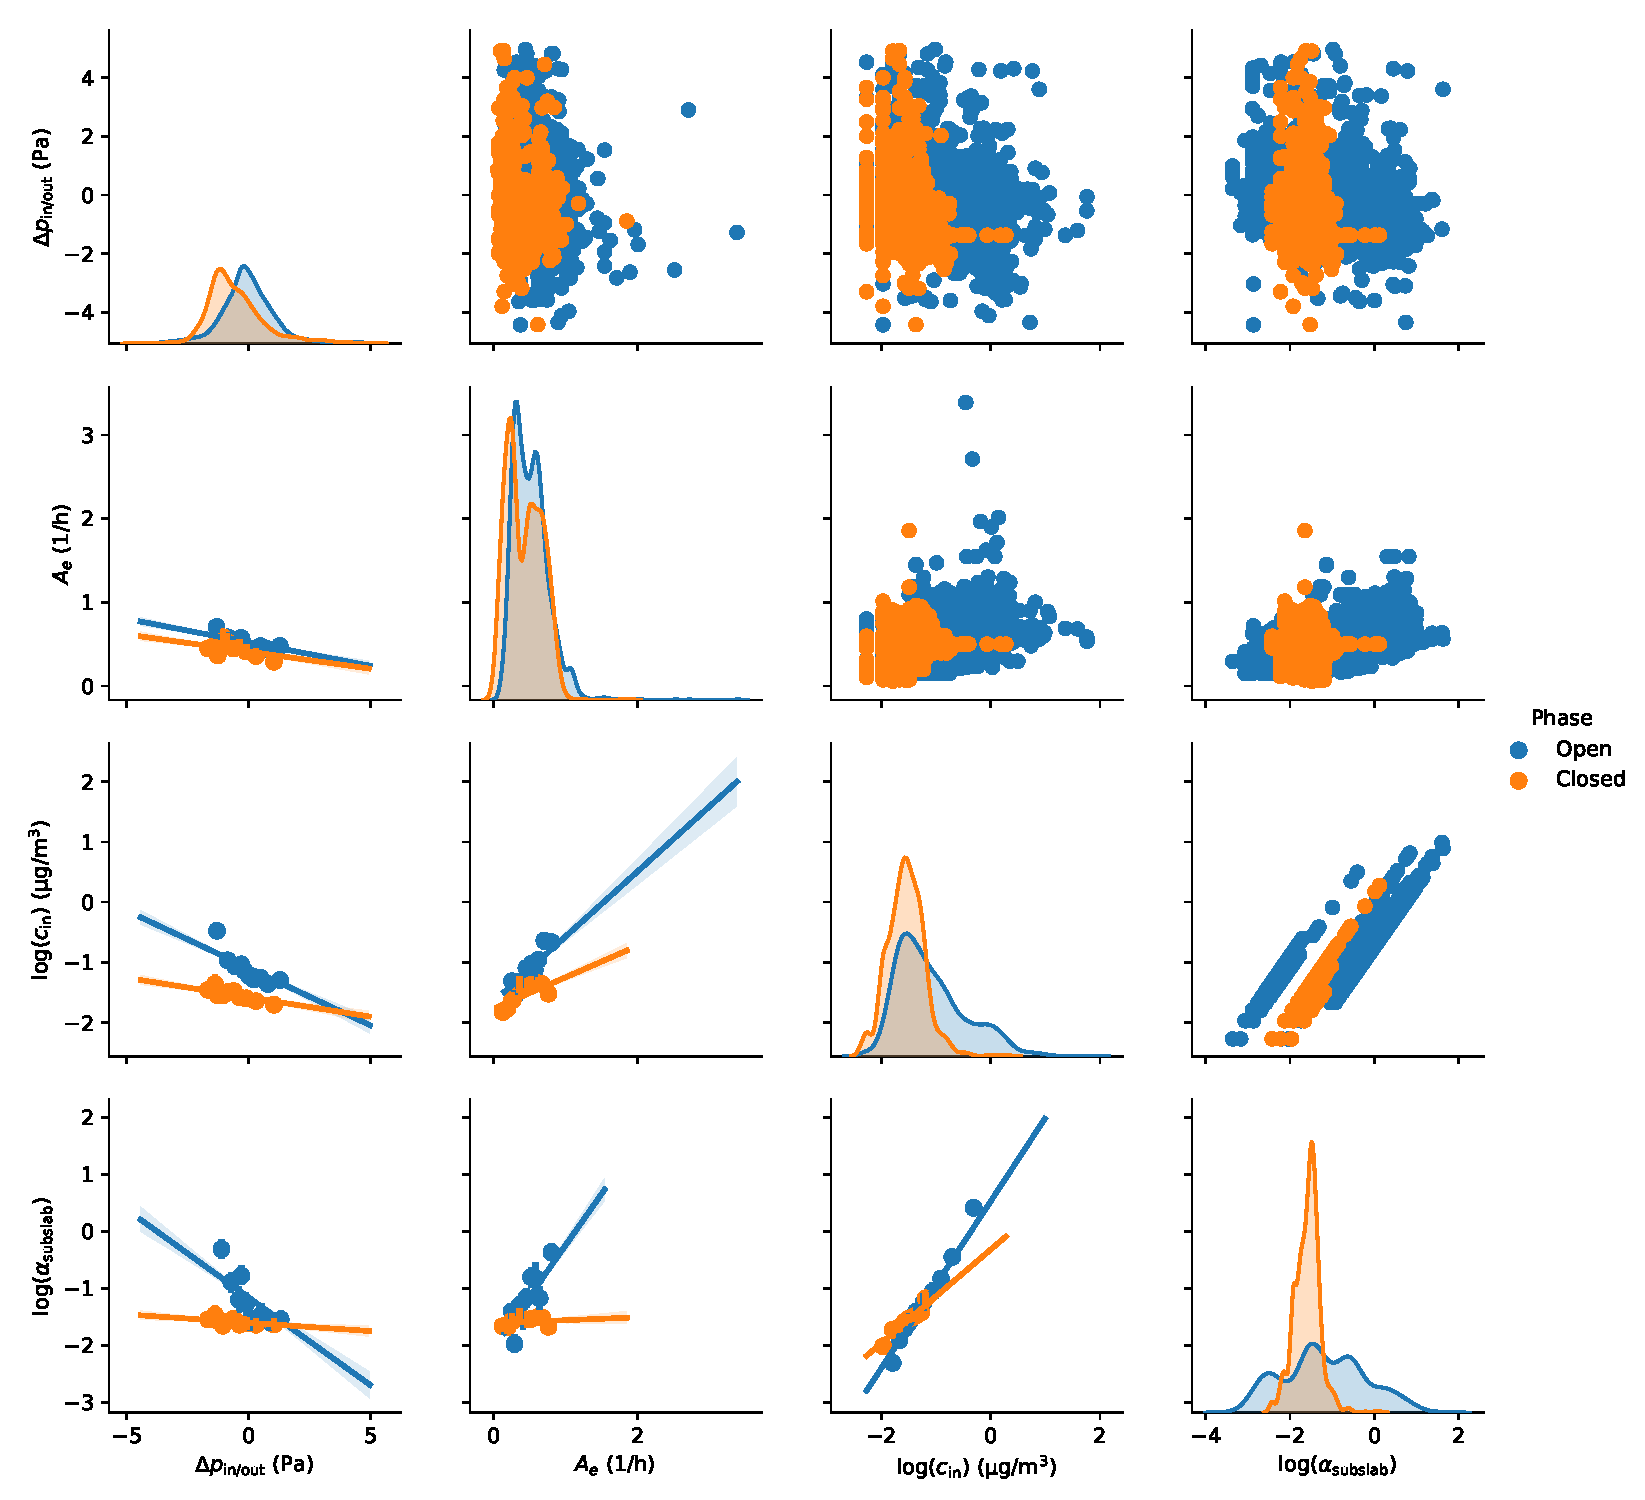
\includegraphics[width=\textwidth]{asu_phase.pdf}
	\end{minipage}
	%\hspace{3cm}
	\begin{minipage}[c]{0.49\textwidth}
		\centering
    \caption{ }
    \label{fig:indianapolis_species}
    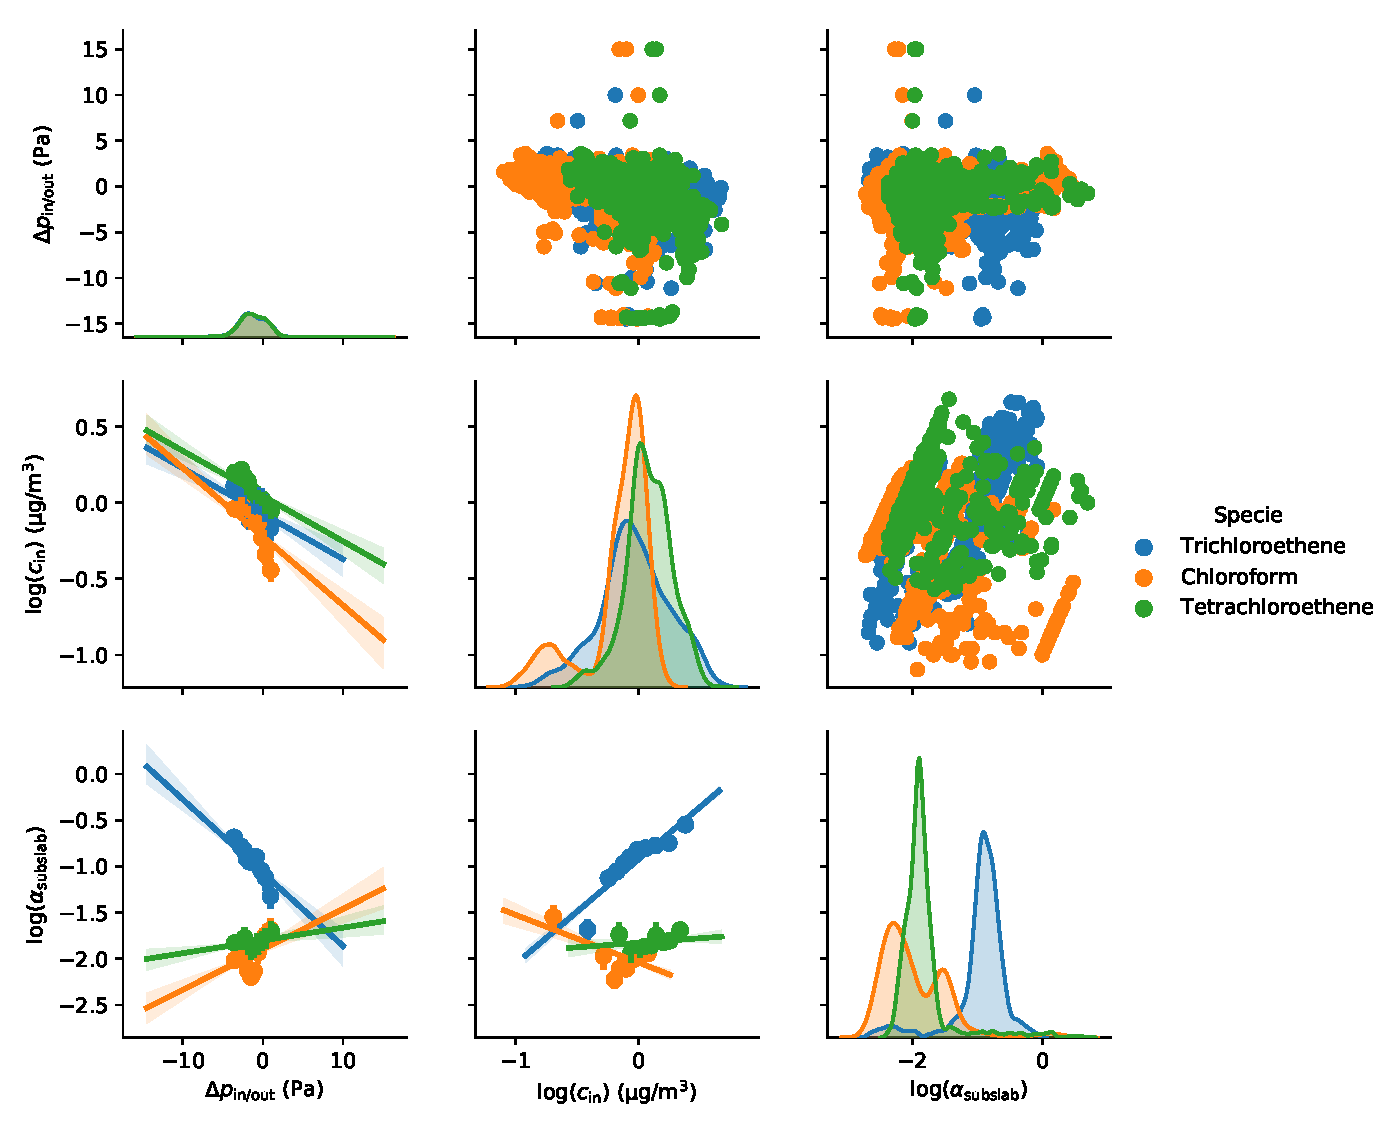
\includegraphics[width=\textwidth]{indianapolis_species.pdf}
	\end{minipage}
\end{figure}


\subsection{Seasonal Variability}

\begin{figure}[htb!]
  \caption{ }
  \label{fig:seasonal_analysis}
  % ASU/North Island plot
  \begin{subfigure}{0.49\textwidth}
    \centering
    \caption{ }
    \label{fig:seasonal_analysis_asu}
    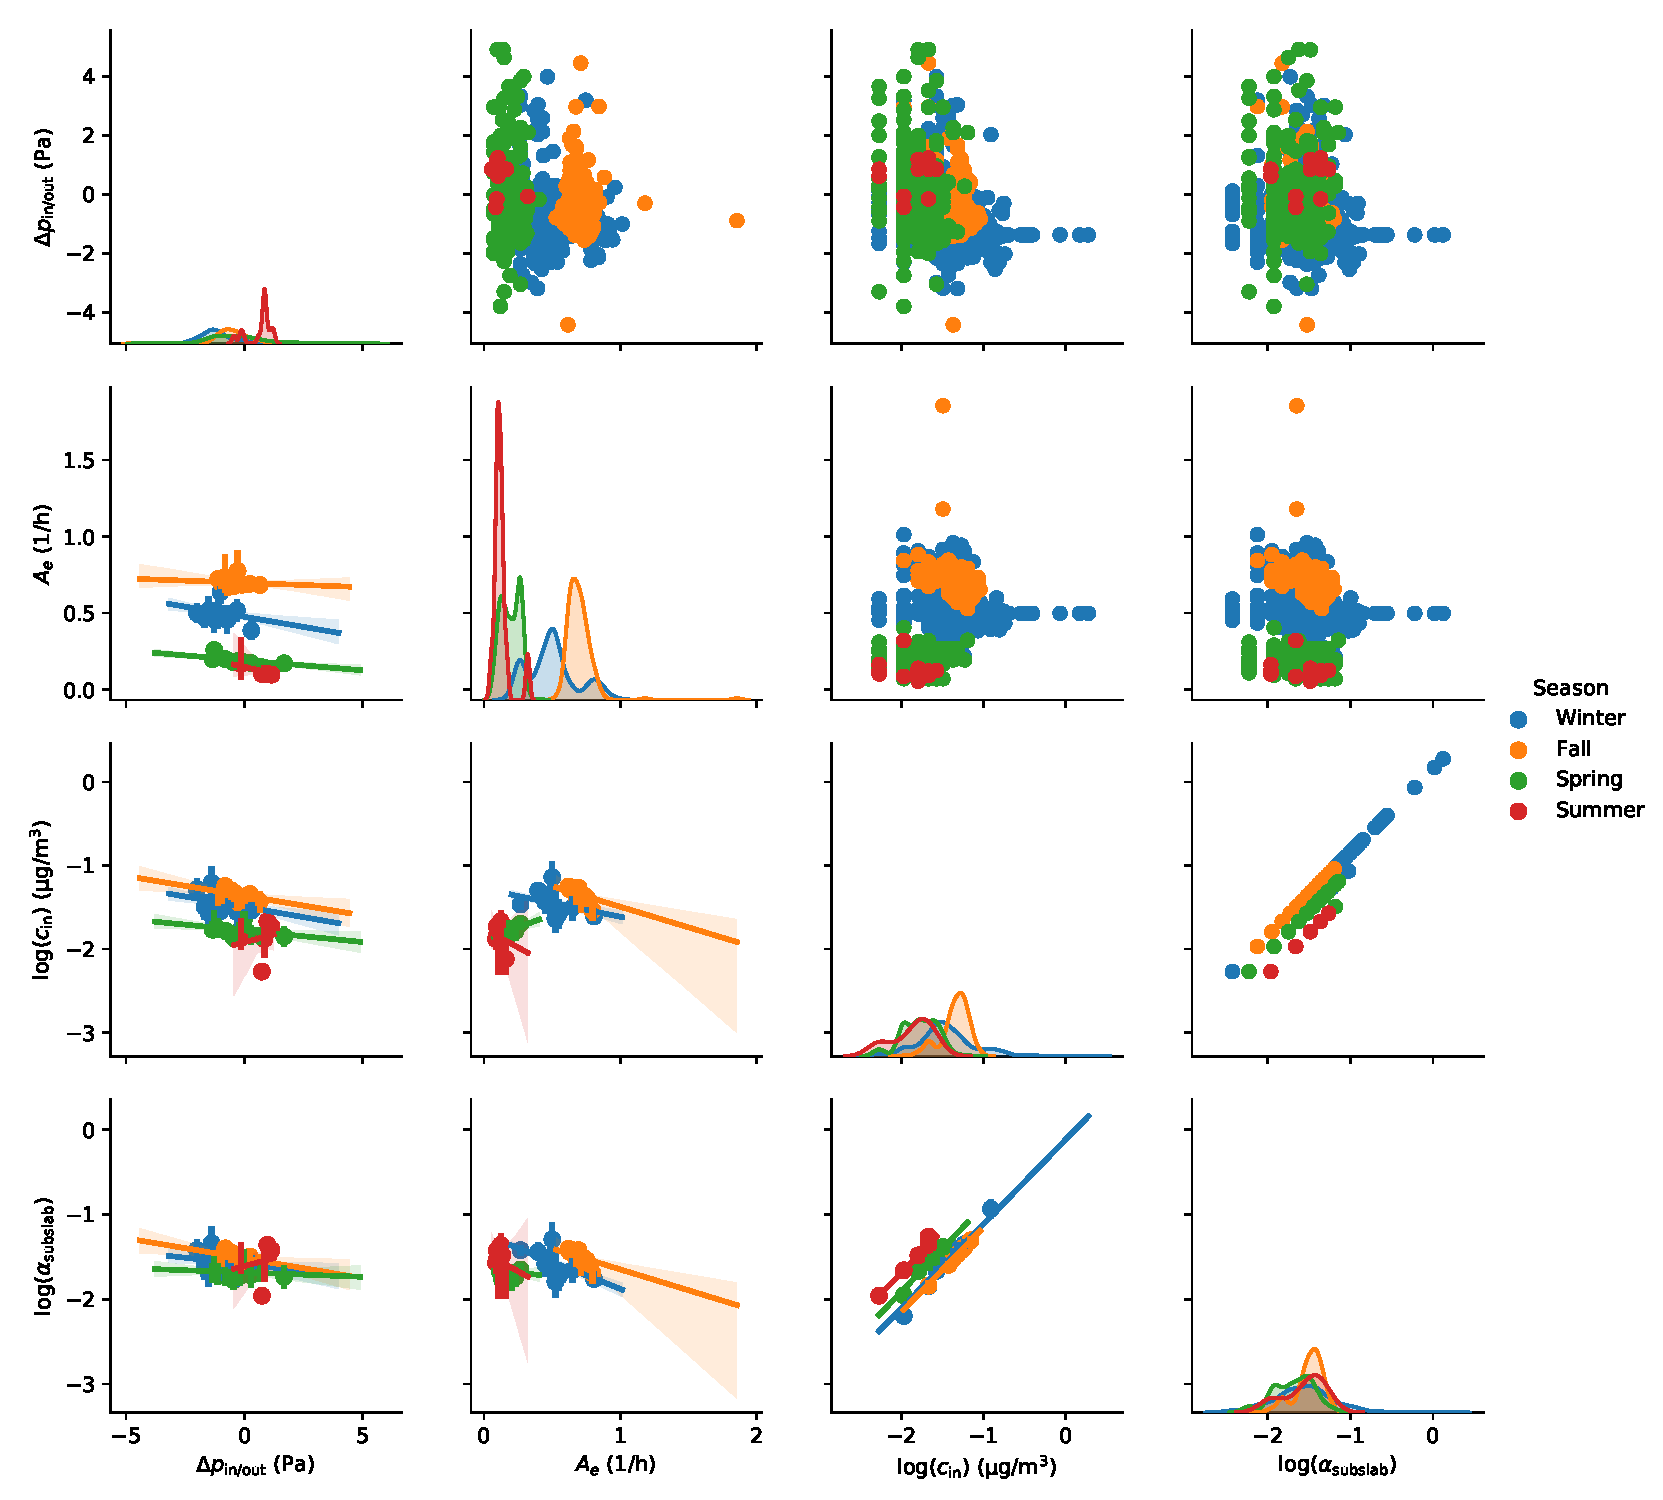
\includegraphics[width=\textwidth]{asu_closed_season.pdf}
  \end{subfigure}
  % Indianapolis plot
  \begin{subfigure}{0.49\textwidth}
    \centering
    \caption{ }
    \label{fig:seasonal_analysis_indianapolis}
    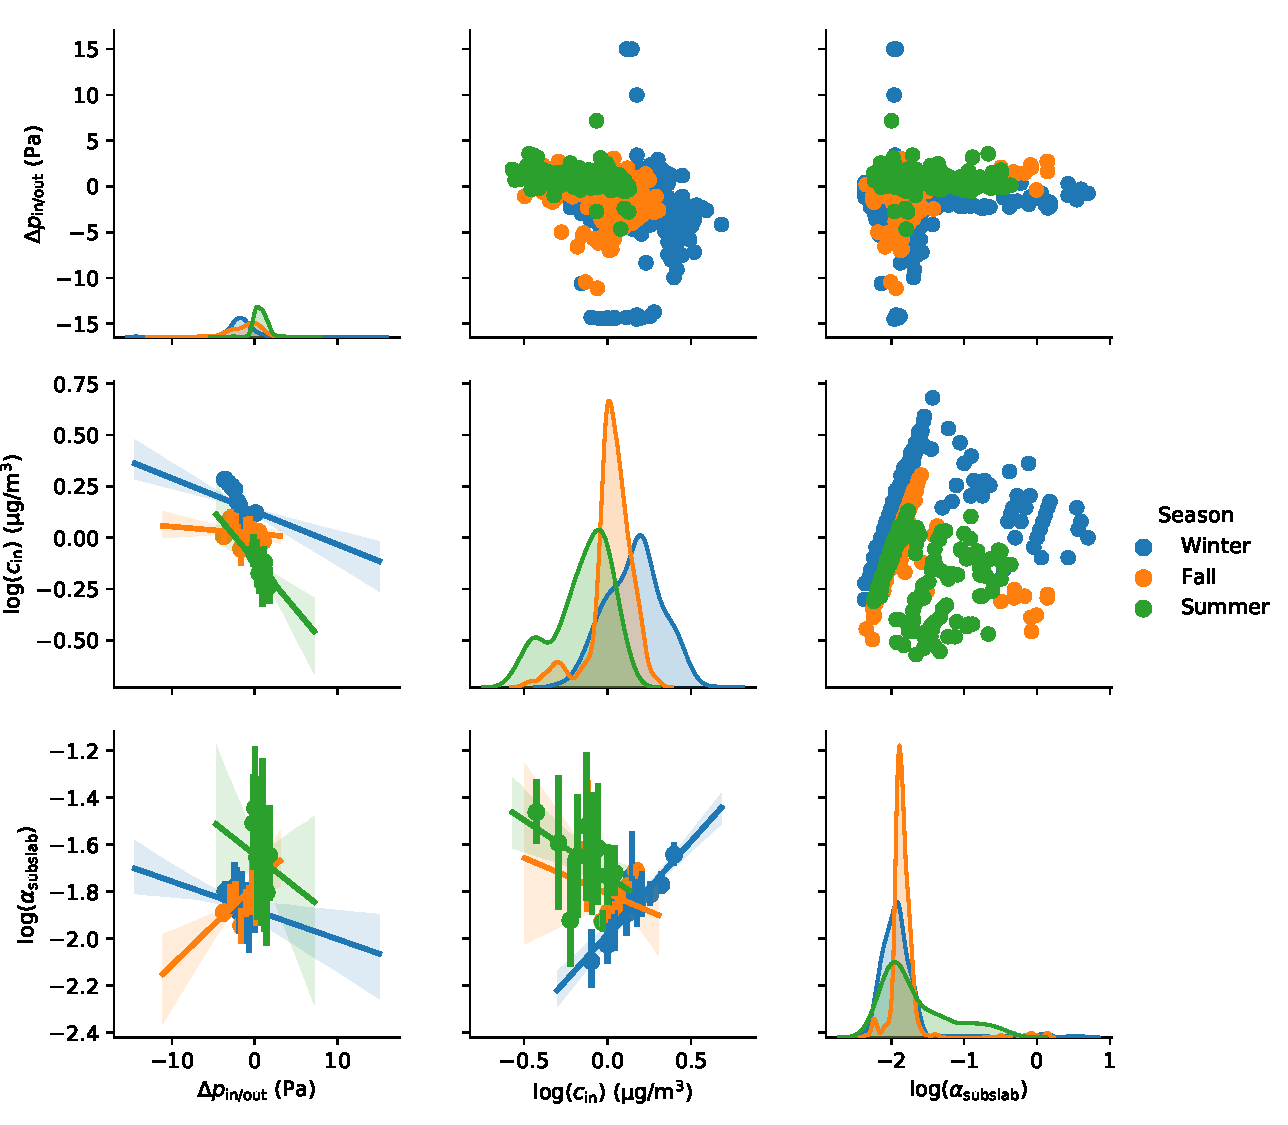
\includegraphics[width=\textwidth]{indianapolis_pce_season.pdf}
  \end{subfigure}
\end{figure}

\subsection{Maximum Change in Indoor Air Contaminant Concentration}

\begin{figure}[!h]
	\centering
	\begin{minipage}[c]{0.49\textwidth}
		\centering
    \caption{ }
    \label{fig:resampling}
    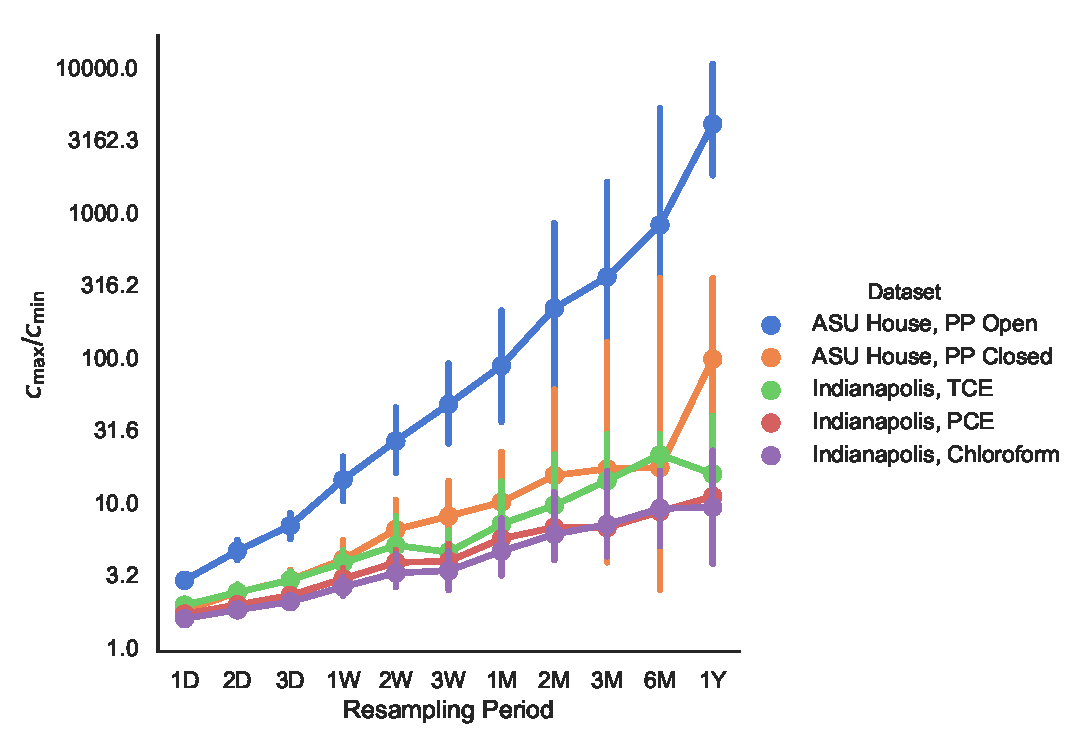
\includegraphics[width=\textwidth]{temporal_variability/resampling.pdf}
	\end{minipage}
	%\hspace{3cm}
	\begin{minipage}[c]{0.49\textwidth}
		\centering
    \caption{Simulated cases}
    \label{fig:land_drain_scenarios}
    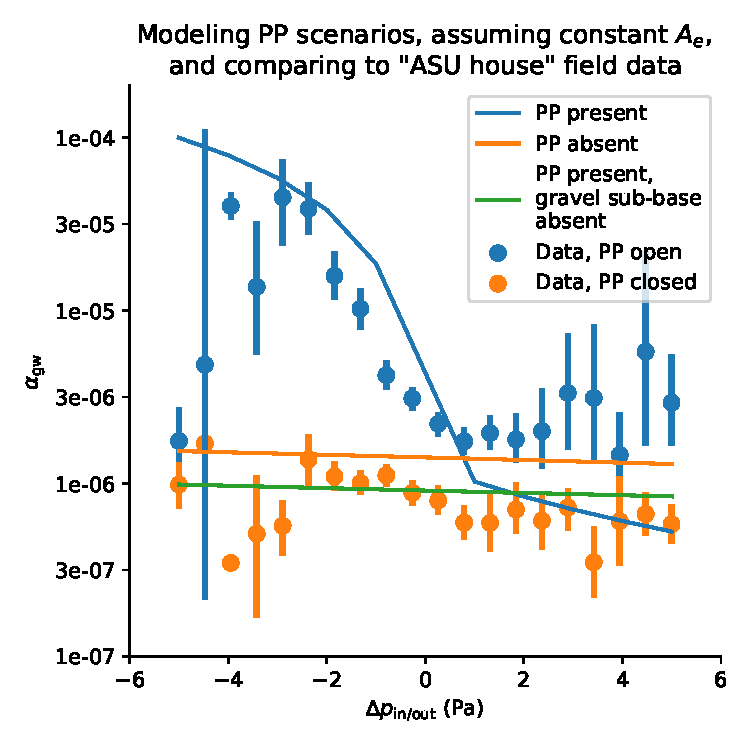
\includegraphics[width=\textwidth]{land_drain_scenarios.pdf}
	\end{minipage}
\end{figure}



\subsubsection{Modeling Indoor Air Variability}

\begin{figure}[htb!]
  \caption{ }
  \label{fig:simulation_sampling}
  % ASU/North Island plot
  \begin{subfigure}{0.49\textwidth}
    \centering
    \caption{ }
    \label{fig:simulation_sampling_pp_open}
    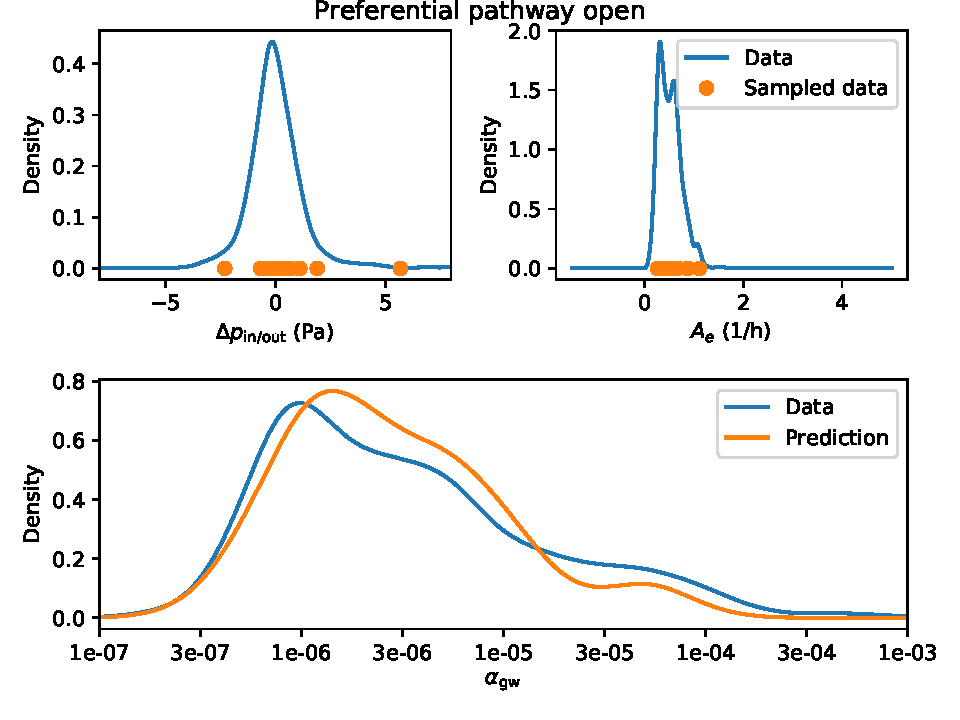
\includegraphics[width=\textwidth]{sampling_simulation_pp_open.pdf}
  \end{subfigure}
  % Indianapolis plot
  \begin{subfigure}{0.49\textwidth}
    \centering
    \caption{ }
    \label{fig:simulation_sampling_pp_closed}
    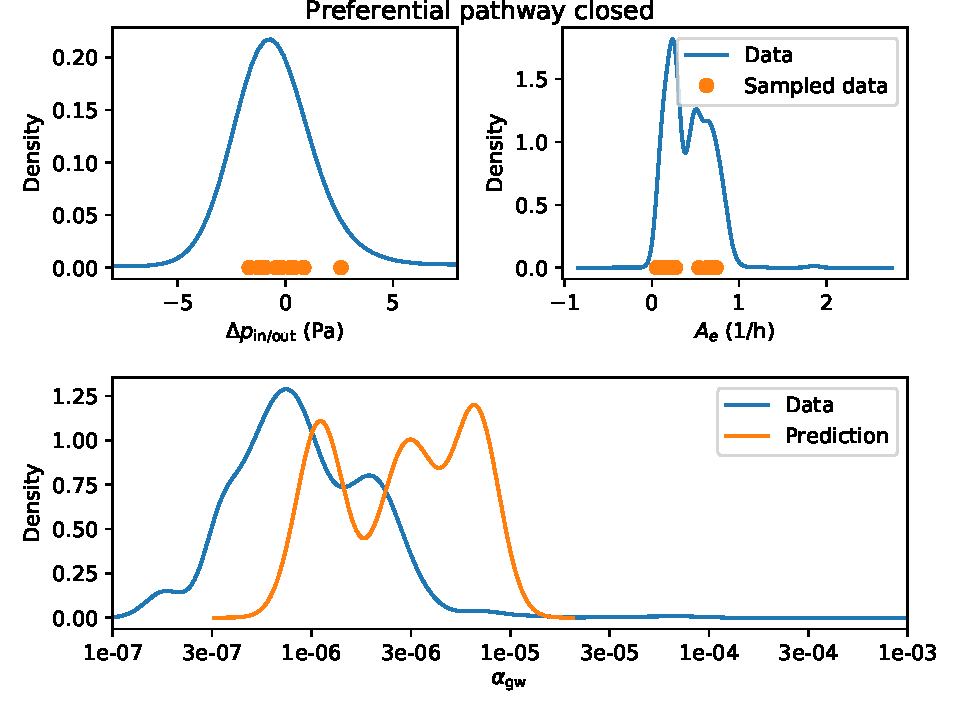
\includegraphics[width=\textwidth]{sampling_simulation_pp_closed.pdf}
  \end{subfigure}
\end{figure}


\begin{acknowledgement}
  This project was supported by grant ES-201502 from the Strategic Environmental Research and Development Program and Environmental Security Technology Certification Program (SERDP-ESTCP).
\end{acknowledgement}

\bibliography{library}

\end{document}
